\section{The On-the-Fly Decision Procedure}\label{sec:correct}

We turn the calculus of \S\ref{sec:tableau} into an algorithm (\S\ref{ss:otf}) and prove it
terminates in deterministic exponential time (\S\ref{ss:term}), is sound for all of TCTL, and is
complete over the non-punctual fragment (\S\ref{ss:sound}). Throughout, $\varphi$ is the input
formula, $n=|\FL(\varphi)|$, and $M$ the largest constant in its intervals.

\subsection{The algorithm}\label{ss:otf}

Write $\mathcal M^{*}$ for the largest successful marking of \S\ref{ss:loop}. Both clauses of that
definition are monotone, so $\mathcal M^{*}$ is the greatest fixpoint of the operator that deletes
from a candidate set every node violating one, and the tableau succeeds iff the root lies in
$\mathcal M^{*}$. Algorithm~\ref{alg:otf} decides that membership.

Nothing is enumerated in advance. \Expand{} applies the rules of \S\ref{ss:rules} to a node the
first time the search reaches it and returns the recorded verdict of an already-retired
$\cong_M$-equal node otherwise, so each node is expanded at most once and the graph exists only as
far as the search has demanded it. The traversal carries Tarjan's indices; we use that algorithm as
a black box and restate none of it. When a component closes it is eliminated at once by
Algorithm~\ref{alg:elim} and its nodes \emph{retire} with a final verdict, after which they are never revisited.
What the procedure holds at any moment is the current search path together with the verdicts of
retired nodes --- never the graph of Lemma~\ref{lem:finiteness}.

Line~\ref{alg:prune} is what keeps the search demand-driven rather than merely lazy. A child settles
its parent when the parent is an $\ORn$-node and the child holds, or an $\ANDn$-node and it fails;
the parent then retires immediately and its remaining children are \emph{never built}. Without it
the procedure would visit every reachable node even when the first child already exhibits a witness.
The guard $\mathrm{top}(\Stack)=v$ is what makes this well defined: an earlier child may have left
members of $v$'s own component above $v$ on Tarjan's stack, and $v$ cannot be lifted out from under
them. Lemma~\ref{lem:prune} shows the pruning changes no verdict.

\begin{algorithm}[!htb]
\DontPrintSemicolon
\SetAlgoLined
\SetKwInOut{Input}{input}
\SetKwInOut{Output}{output}
\SetKwInOut{State}{state}
\SetKwProg{Fn}{procedure}{}{end}
\SetKwProg{Fun}{function}{}{end}

\Input{$\varphi$ in negation normal form}
\Output{\SAT{} or \UNSAT}
\State{$\val[v]\in\{\top,\bot,?\}$ initially $?$ (undecided);
       $\idx[v],\low[v]\in\Nat\cup\{\bot\}$ and $\onstk[v]$ initially $\bot$, \textsf{false};
       Tarjan's stack $\Stack$ initially empty; counter $\cnt\in\Nat$ initially $0$}
\BlankLine

\Fn{\Decide{$\varphi$}}{
  $N_0\gets\tup{\{\varphi\}}{\emptyset}{\mathbf 0}{\emptyset}{\emptyset}$\;
  \Explore{$N_0$}\;
  \Return{\SAT{} if $\val[N_0]=\top$, else \UNSAT}\;
}
\BlankLine

\Fn{\Explore{$v$}}{
  $\idx[v]\gets\low[v]\gets\cnt$; \ $\cnt\gets\cnt+1$;
    \ $\mathrm{push}(\Stack,v)$; \ $\onstk[v]\gets\textsf{true}$\;
  $\ch[v]\gets$ \Expand{$v$} \tcp*{rules of \S\ref{ss:rules}, memoised on $\cong_M$}
  \ForEach{$w\in\ch[v]$}{
    \uIf{$\idx[w]=\bot$}{
      \Explore{$w$}; \ $\low[v]\gets\min(\low[v],\low[w])$ \tcp*{tree edge}
    }
    \ElseIf{$\onstk[w]$}{
      $\low[v]\gets\min(\low[v],\idx[w])$ \tcp*{back edge}
    }
    \lIf{\Settles{$v,w$} \textnormal{\textbf{and}} $\mathrm{top}(\Stack)=v$\label{alg:prune}}{
      \Retire{$v,\val[w]$}; \Return}
  }
  \If{$\low[v]=\idx[v]$}{
    $C\gets$ pop $\Stack$ down to and including $v$; \ $\onstk[u]\gets\textsf{false}$ for $u\in C$\;
    \Eliminate{$C$}\;
  }
}
\BlankLine

\Fun{\Settles{$v,w$}}{
  \Return{$\val[w]\neq{?}$ \textnormal{\textbf{and}} $\big(\val[w]=\bot$ if $v$ is an
          $\ANDn$-node, else $\val[w]=\top\big)$}\;
}
\BlankLine

\Fn{\Retire{$v,b$}}{
  $\val[v]\gets b$; \ $\onstk[v]\gets\textsf{false}$; \ $\mathrm{pop}(\Stack)$\;
}
\caption{On-the-fly satisfiability test: demand-driven traversal. Retiring at
line~\ref{alg:prune} leaves $v$'s remaining children unbuilt.}\label{alg:otf}
\end{algorithm}

\begin{algorithm}[!htb]
\DontPrintSemicolon
\SetAlgoLined
\SetKwProg{Fn}{procedure}{}{end}
\Fn{\Eliminate{$C$}}{
  $A\gets C$\;
  $\Out\gets\{w\notin C\mid w\in\ch[v]$ for some $v\in C$, $\val[w]=\top\}$ \tcp*{final}
  \Repeat{$A$ is unchanged}{
    $A\gets A\setminus\{v\in A\mid v$ closed$\}$\;
    $A\gets A\setminus\{v\in A\mid v$ an $\ORn$-node, $\ch[v]\cap(A\cup\Out)=\emptyset\}$\;
    $A\gets A\setminus\{v\in A\mid v$ an $\ANDn$-node, $\ch[v]\not\subseteq A\cup\Out\}$\;
    $G\gets\{v\in A\mid \ch[v]\cap\Out\neq\emptyset\}\cup
      \bigcup\{T\mid T$ a time-progressing SCC of $A\}$\;
    $A\gets A\setminus\{v\in A\mid v$ has no $A$-path to $G\}$ \tcp*{\ref{M1}}
    \ForEach{until $\mu$ with $\mu^\bullet$ active in $A$}{
      $G_\mu\gets\{v\in A\mid v$ takes \ruleref{Ustop} for $\mu\}\cup
        \{v\in A\mid \ch[v]\cap\Out$ carries $\mu^\bullet\}$\;
      $A\gets A\setminus\{v\in A\mid \mu^\bullet$ at $v$, no $\mu^\bullet$-path to $G_\mu\}$
        \tcp*{\ref{M2}}
    }
  }
  $\val[v]\gets[\,v\in A\,]$ \textnormal{\textbf{for all}} $v\in C$\;
}
\caption{Per-component elimination: the greatest fixpoint of \S\ref{ss:loop} restricted to $C$,
evaluated against the already-final verdicts in $\Out$.}\label{alg:elim}
\end{algorithm}


Two structural facts make \Eliminate{} local. The first is the Tarjan invariant, which we use but do
not restate: when a component $C$ is popped, every child of a node of $C$ lying outside $C$ has
already retired, since children are expanded before their parent completes and a child still on the
stack would drag the lowlink of $C$'s root below its index. Hence $\Out$ is well defined and its
verdicts are final. The second is that $C$ is a \emph{maximal} strongly connected set, so no path
leaving $C$ ever returns to it.

\begin{lemma}[Pruning]\label{lem:prune}
Suppose $\val[w]$ is final and \Settles{$v,w$} holds. Then $\val[v]=\val[w]$ in $\mathcal M^{*}$, and
leaving the remaining children of $v$ unexpanded changes $\mathcal M^{*}$ at no node.
\end{lemma}
\begin{proof}
That $\val[v]=\val[w]$ is the structural clause of \S\ref{ss:loop} alone: an $\ORn$-node with a child
in $\mathcal M^{*}$ is in it, an $\ANDn$-node with a child outside it is out.

For the second claim, note that the explored subgraph is closed under successors \emph{except} at
retired nodes, so a path of $\mathcal M^{*}$ that uses an unexpanded child of $v$ passes through $v$
itself. If $\val[v]=\bot$ then $v\notin\mathcal M^{*}$ and no path of $\mathcal M^{*}$ uses $v$ at
all. If $\val[v]=\top$ then $v\in\mathcal M^{*}$, so $v$ already satisfies \ref{M1}, and \ref{M2} for
every pursuit active at $v$; a node $u$ reaching $v$ therefore obtains its own witness by prefixing
the path from $u$ to $v$ --- for \ref{M2} the prefix carries $\mu^\bullet$ exactly when $\mu^\bullet$
is active at $v$, and a path that abandons $\mu^\bullet$ is not admissible in either reading. Since
no path leaving a maximal component returns to it, removing $v$'s remaining out-edges also leaves
every component classification unchanged.
\end{proof}

\noindent
The pruning is what earns the name: the procedure stops at the first witness rather than exhausting
the reachable graph, and by Lemma~\ref{lem:prune} it does so without changing a single verdict.

\begin{lemma}[Locality]\label{lem:locality}
Let $S$ be an SCC and suppose $\val[c]=[\,c\in\mathcal M^{*}\,]$ for every child $c\notin S$ of a
node of $S$. Then $\mathcal M^{*}\cap S$ is the largest $A\subseteq S$ closed under the deletions of
\Eliminate{$C$}.
\end{lemma}
\begin{proof}
A path of $\mathcal M^{*}$ issued from $N\in S$ either stays in $S$ or leaves it once and for all, at
some $c\in\mathcal M^{*}\setminus S$. In the first case a witness for \ref{M1}--\ref{M2} lies inside
$S$, which is what the two deletions search for. In the second, $c$ lies in $\mathcal M^{*}$ and so
already satisfies \ref{M1}, and \ref{M2} for $\mu^\bullet$ whenever $\mu^\bullet$ is active at $c$;
prefixing the path from $N$ to $c$ turns either witness into one for $N$, which is what the
alternatives ``child in $\Out$'' record. Conversely every deletion of \Eliminate{} is an instance of
a clause of \S\ref{ss:loop}. The two systems have the same post-fixpoints within $S$,
hence the same greatest one.
\end{proof}

\noindent
Deleting a node can disconnect $A$, and a component that is no longer strongly connected no longer
supports the cycle its classification assumed, so the decomposition is recomputed each round; the
next lemma makes that step exact and linear.

\begin{lemma}[Progress]\label{lem:progress}
A strongly connected set $T$ of nodes with at least one internal edge carries a time-progressing
cycle iff \emph{(a)} some node of $T$ is a \ruleref{Delay}-successor, and \emph{(b)} every clock is
either reset at some node of $T$ or unbounded at every node of $T$.
\end{lemma}
\begin{proof}
($\Leftarrow$) As $T$ is strongly connected, concatenating paths yields a cycle $C$ through the node
of (a) and through one reset node of every clock that (b) resets in $T$. $C$ crosses a
\ruleref{Delay} step, so it elapses positive time, and every clock is reset on $C$ or, by (b),
unbounded throughout $T\supseteq C$; so $C$ is time-progressing.
($\Rightarrow$) Let $C\subseteq T$ be time-progressing. It elapses positive time, hence crosses a
\ruleref{Delay} step, giving (a). For (b), let $x$ be reset at no node of $T$, hence at none of $C$;
$C$ being time-progressing then forces $x$ unbounded at every node of $C$. For $u\in T$, strong
connectivity gives a path inside $T$ from a node of $C$ to $u$ along which $x$ is never reset, so its
value only grows and, being already above $M$, stays extrapolated; thus $x$ is unbounded at $u$.
\end{proof}

\begin{lemma}[Adequacy]\label{lem:alg}
Algorithm~\ref{alg:otf} retires every node with $\val[N]=[\,N\in\mathcal M^{*}\,]$; in
particular it returns \SAT{} iff the root lies in $\mathcal M^{*}$.
\end{lemma}
\begin{proof}
Components are popped in reverse topological order, so by the Tarjan invariant each call of \Eliminate{}
meets the hypothesis of Lemma~\ref{lem:locality}. Inside $S$ the loop is the deletion operator of
\S\ref{ss:loop} restricted to $S$, exact by Lemma~\ref{lem:progress} and monotone
decreasing on a finite set, so it reaches the greatest post-fixpoint, which is $\mathcal M^{*}\cap S$.
\end{proof}

\subsection{Termination and Complexity}\label{ss:term}

\begin{lemma}\label{lem:finiteness}
The number of distinct nodes the procedure can generate is bounded above by
$2^{O(n)}\cdot M^{O(n^2)}$.
\end{lemma}
\begin{proof}
The propositional components $\Gamma,\Ctx$ range over subsets of $\FL(\varphi)$, hence $2^{O(n)}$
choices each; the clock map $\obligations$ over $2^{O(n)}$ assignments and $\Deadline$ over $2^{O(n)}$
choices. The cover rule allocates one formula-clock per timed subformula, bounded by $O(n)$. A
canonical $\cong_M$-zone over $K$ clocks is a $(K{+}1)^2$ DBM whose finite entries lie in
$\{-M,\dots,M\}\times\{<,\le\}$, giving $M^{O(K^2)}\le M^{O(n^2)}$ distinct zones. Multiplying the
components yields $2^{O(n)}\cdot M^{O(n^2)}$.
\end{proof}

\begin{theorem}\label{thm:complexity}
Satisfiability of non-punctual TCTL is \textsc{ExpTime}-complete, and Algorithm~\ref{alg:otf} decides
it in time $2^{\mathrm{poly}(n)}$.
\end{theorem}
\begin{proof}
Let $m=2^{O(n)}\cdot M^{O(n^2)}$ be the bound of Lemma~\ref{lem:finiteness}; as the encoding of $M$
occupies at most $n$ input symbols, $\log m=O(n)+O(n^2)\log M=\mathrm{poly}(n)$. The explored graph
has at most $m$ nodes and $m^2$ edges, and memoisation on $\cong_M$-classes expands each node at most
once --- which is what avoids the doubly exponential blow-up of the naive ancestor-only unfolding ---
so the traversal halts, Tarjan adding linear overhead. Retiring a node at
line~\ref{alg:prune} only removes expansions, so it can only lower these counts.

Each $\Sat_{\Ctx}(\mu)$ is a least ($\mathbf U$) or greatest ($\mathbf R$) fixpoint of a monotone map
on unions of $\cong_M$-zones, at most $M^{O(n^2)}$ in number; by Knaster--Tarski it exists and
monotone iteration reaches it in as many steps, each a polynomial number of DBM operations, with a
factor $O(n)$ over $\FL(\varphi)$.

It remains to charge the eliminations. Each round of \Eliminate{$C$} deletes a node or stops, so there are
at most $|S|$ rounds; a round performs one decomposition of $A$, one backward reachability for
\ref{M1} and one per pursued until for \ref{M2}, each linear in the subgraph, and there are $O(n)$
untils. A component costs $O(n\,|S|\,(|S|+|E_S|))$, and the components partition the nodes, so all
eliminations together cost $\mathrm{poly}(m)$. The procedure runs in $2^{\mathrm{poly}(n)}$.
Hardness is inherited: fixing every interval to $[0,\infty)$ it decides CTL satisfiability, which is
\textsc{ExpTime}-hard~\cite{Clarke99}.
\end{proof}

\subsection{Soundness and Completeness}\label{ss:sound}

Four lemmas support the two constructions: one makes the zones realisable as delays, one reconciles
the discrete induction with the dense semantics, one supplies time divergence, and one relates
$\Sat_{\Ctx}$ to truth.

\begin{lemma}\label{lem:feasible}
Let $N_0,\dots,N_k$ be a finite path of $\mathcal{M}$ with non-empty zones. For every $\nu_k\in Z_k$
there are $\nu_0\in Z_0,\dots,\nu_{k-1}\in Z_{k-1}$ and positive delays realising every step.
\end{lemma}
\begin{proof}
Each operation used along a path (intersection and guards, reset, time-successor and
$\cong_M$-canonicalisation) admits back-propagation, non-empty precisely because the successor
valuation lies in its image~\cite{Bouyer05TimedAutomata}; threading backward from $\nu_k$ gives the
assignment.
\end{proof}

\begin{lemma}\label{lem:stability}
Along a delay step $(s,\nu)\xrightarrow{t}(s,\nu+t)$ that crosses no integer hyperplane $x=b$
($b\le M$), the truth of every subformula of $\varphi$ is constant over the relatively-open segment
$(s,\nu+t')$, $t'\in(0,t)$.
\end{lemma}
\begin{proof}
Crossing no hyperplane $x=b$ with $b\le M$, no clock crosses an integer at or below $M$, so no integer
part changes and no fractional ordering wraps; clocks already above $M$ are identified by
extrapolation and their exact values are immaterial. All $(s,\nu+t')$ lie in one clock region, and
TCTL truth is constant on a region~\cite{AlurCourcoubetisDill1990,Bouyer05TimedAutomata}.
\end{proof}
\noindent
The endpoints, where a clock sits exactly on a hyperplane, are nodes of their own by the integer split
of \ruleref{Delay}: a guard $x_\mu\in\kI$ is then tested against $x_\mu=b$, and whether it holds there
is decided by the strictness flag of $\kI$'s endpoint.

\begin{lemma}\label{lem:nonzeno}
A candidate loop $N_i\equiv N_j$ has a non-Zeno unfolding iff it is \emph{time-progressing}: it admits
positive total elapsed time and every clock is either reset on the segment or extrapolated above $M$,
hence unbounded. When it is, a run exists in which every iteration elapses the same positive amount.
\end{lemma}
\begin{proof}
($\Rightarrow$) By contraposition, suppose the loop is not time-progressing. Either it elapses no
time, and infinitely many traversals take zero time in total; or some clock $x$ is neither reset on
the segment nor extrapolated above $M$, so it retains a finite bound $x\le c$ with $c\le M$ in the
zones of the loop. In the latter case $x$ is unreset, hence increases by exactly the delay elapsed on
each traversal, and the bound is enforced at every node; the delays of all iterations therefore sum to
at most $c-\nu(x)$, and infinitely many delays with a finite sum converge. Either way the unfolding is
Zeno.
($\Leftarrow$) Lemma~\ref{lem:feasible} yields a traversal of the loop with some $\delta>0$. Since
$N_i\equiv N_j$ no rule distinguishes the two visits, so the traversal repeats; no budget depletes
either, each clock being reset on the segment or extrapolated above $M$, hence unbounded. So $\delta$
recurs at every iteration and $\sum_k t_k\ge\sum_k\delta=\infty$.
\end{proof}

\begin{lemma}\label{lem:sat}
Let $\mu$ be demanded at $N$ under $\Ctx$, $\nu\in Z_N$, and let $\mathcal{T}$ be the TTS read off a
successful marking containing $N$, with $s_N$ the location of $N$. Let $\mathcal{T}'$ be any TTS with
configuration $(s,\nu)$ satisfying $\Ctx$. Then
\[
  (i)\ \nu\in\Sat_{\Ctx}(\mu)\ \Longrightarrow\ \mathcal{T},(s_N,\nu)\models\mu,
  \qquad
  (ii)\ \mathcal{T}',(s,\nu)\models\mu\ \Longrightarrow\ \nu\in\Sat_{\Ctx}(\mu)
\]
\end{lemma}
\begin{proof}
By Lemma~\ref{lem:stability} the truth of every subformula is constant along the open segment between
consecutive nodes, so we may argue at nodes. Write $\Sat_{\Ctx}(\mu)^{k}$ for the valuations obtained
after $k$ unfoldings: for an until those reaching a base child within $k$ steps, growing from
$\emptyset$; for a release those violating the obligation at no step among the first $k$, shrinking
from the universal zone. By construction $\nu\in\Sat_{\Ctx}(\mu)$ means $\nu\in\Sat_{\Ctx}(\mu)^{k}$
for some $k$ in the first case and every $k$ in the second, and both sequences stabilise in finitely
many steps.

\textit{\lemitem{lem:sat}{i}} The runs of $\mathcal{T}$ from $(s_N,\nu)$ are the pursuit paths from
$N$, the discrete edges of $\mathcal{T}$ being the pursuits' $\EX/\AX$-successors (\ruleref{Cov}
contributes none). For an until, induct on the least $k$ with $\nu\in\Sat_{\Ctx}(\mu)^{k}$. If $k=1$,
$\nu$ lies in a base zone, so \ruleref{Ustop} applies: $\psi$ holds at $(s_N,\nu)$ with
$x_\mu\in\kI$ and \eqref{eq:sat_u} is met at the current position. If $k>1$, $\nu$ matches a
\ruleref{Ugo} child, so $\varphi$ holds and the deferred successors lie in $\Sat_{\Ctx}(\mu)^{k-1}$;
by induction $\mu$ holds at each, and prepending the current position gives a run satisfying
\eqref{eq:sat_u}. The quantifier follows from the child: for $\mathrm{Q}=\mathrm{E}$ one successor is
demanded and the run through it witnesses $\exists\rho$; for $\mathrm{Q}=\mathrm{A}$ all are, and
every run begins with one of them. The deadline in $\Inv(N)$ stops a universal run idling past the
window. For a release the hypothesis gives $\nu\in\Sat_{\Ctx}(\mu)^{k}$ for every $k$; a position
$\pi=(i,\delta)$ of a run from $(s_N,\nu)$ is reached after $i$ discrete steps, so $k=i+1$ gives that
the obligation is not violated at $\pi$, and $\pi$ was arbitrary, which is \eqref{eq:sat_r}.

\textit{\lemitem{lem:sat}{ii}} Here $\mathcal{T}'$ is arbitrary, so we read a path off a run. A run
satisfying \eqref{eq:sat_u} reaches $\psi$ at a position $(i,\delta)$ with $i$ finite; selecting at
each step the branch the run takes gives a path into a base child in $i$ steps, so
$\nu\in\Sat_{\Ctx}(\mu)^{i}$. For $\mathrm{Q}=\mathrm{E}$ one such run suffices; for
$\mathrm{Q}=\mathrm{A}$ every run gives such a path and, the pursuit graph being finitely branching
(each rule has finitely many children, Lemma~\ref{lem:finiteness}), K\"onig's lemma bounds them all by
a single $k$. For a release we show $\nu\in\Sat_{\Ctx}(\mu)^{k}$ by induction on $k$: the obligation
is met at the current position since \eqref{eq:sat_r} holds along the runs of $\mathcal{T}'$, and the
successors inherit the hypothesis.
\end{proof}

\begin{theorem}[Soundness]\label{thm:soundness}
If Algorithm~\ref{alg:otf} returns \SAT{} then $\varphi$ is satisfiable.
\end{theorem}
\begin{proof}
By Lemma~\ref{lem:alg} the root lies in $\mathcal M^{*}$. Read off a witness TA $\mathcal A$: its
locations are the nodes of $\mathcal M^{*}$, labelled by the atoms in $\Gamma$ and carrying $\Inv(N)$
as invariant; its transitions are the AND-children $\mathcal M^{*}$ retains, guarded by
$Z_N\cap\Inv(N)$ for the target $N$, so every $\EX\psi$ obtains a successor satisfying $\psi$ while
each node's $\Ctx$ is imposed on all successors, letting universal obligations constrain the whole
branching. A transition resets $x_\mu$ exactly when its target carries a launch of $\mu$, measuring
the window from the demanding configuration; the residual of a live pursuit crosses without reset.
\ruleref{Delay} generates no transition --- the location is unchanged and only the zone advances, so a
chain of such steps is one continuous elapse within a single location --- and Lemma~\ref{lem:feasible}
supplies valuations and positive delays along any path.

$\mathcal A$ is non-blocking: its only invariants are the until deadlines in $\Inv(N)$, registered by
\ruleref{Cov} on launching a universal until and retired by \ruleref{Ustop}; cap and stop guard derive
from the same interval, so the stop edge is enabled at the cap itself and no configuration is left
with time blocked and no move available.

Let $\mathcal T$ be the TTS induced by $\mathcal A$. Every configuration admits a divergent run: by
\ref{M1} its node reaches inside $\mathcal M^{*}$ a time-progressing cycle, which
Lemma~\ref{lem:nonzeno} unfolds into a run whose iterations each elapse a fixed $\delta>0$, so the
delays past that point sum to infinity. Hence $\mathrm{Runs}^\infty$ is non-empty at every
configuration, which is all the semantics asks of $\mathcal T$; convergent runs it never inspects.

We show $\mathcal T,(s_0,\nu_0)\models\varphi$ by induction on $\varphi$. Booleans follow from
saturation of $\Gamma$ and closure of contradictory nodes, $\EX\psi$ and $\AX\psi$ from the edges and
the context. For a timed modality $\mu$ demanded at $N$ the cover rule succeeded, so
$Z_N\subseteq\Sat_{\Ctx}(\mu)$ and Lemma~\lemitem{lem:sat}{i} gives
$\mathcal T,(s_N,\nu)\models\mu$ for every $\nu\in Z_N$, one zone thereby discharging otherwise
uncountably many onsets of $\mu$. An existential until is witnessed by the pursuit path \ref{M2}
supplies, extended past its \ruleref{Ustop} by a divergent run; a universal one cannot be evaded,
since $\Inv(N)$ blocks time at $\sup\kI$ and the pursuit rides every successor until stopped.
Lemma~\ref{lem:stability} lifts each conclusion to the dense positions between nodes.
\end{proof}

\begin{theorem}[Completeness]\label{thm:completeness}
If $\varphi$ is satisfiable and non-punctual then Algorithm~\ref{alg:otf} returns \SAT.
\end{theorem}
\begin{proof}
Let $\mathcal T,(s_0,\nu_0)\models\varphi$ with $\mathcal T$ non-Zeno. Build a marking by reading it
off $\mathcal T$, maintaining at each node a configuration of $\mathcal T$ whose valuation lies in the
node's zone and which satisfies its $\Gamma$ and $\Ctx$. At an OR-node a consistent child exists in
each case: for \ruleref{Disj}, $\mathcal T$ satisfies a disjunct; for \ruleref{Covstar},
$\mathcal T,(s,\nu)\models\mu$ gives $\nu\in\Sat_{\Ctx}(\mu)$ by Lemma~\lemitem{lem:sat}{ii}, so $\nu$
lies in some component of $Z\cap\Sat_{\Ctx}(\mu)$; for \ruleref{Uunf}, either the witness is at the
current position with $x_\mu\in\kI$, giving \ruleref{Ustop}, or it is strictly later, so $\varphi$
holds now and \ruleref{Ugo} applies; for \ruleref{Rsplit}, the before-part's continue child demands
nothing, and in the window $\psi$ holds --- no earlier $\varphi$ has released $\mu^\bullet$, or it
would not still be carried. At an AND-node, realise every demanded $\EX\psi$ by a discrete successor
of $\mathcal T$ satisfying $\psi$ and recurse on all of them; the context holds at each because
$\mathcal T$ meets its $\AX$-obligations. Every chosen zone intersection is non-empty, witnessed by
the model's valuations, so no selected node closes. A persistent context re-imposes $\mu$ at a
continuum of onsets, but both sides of $Z\subseteq\Sat_{\Ctx}(\mu)$ are finite unions of zones, so one
inclusion settles them together.

The result $\mathcal M$ is a marking; we check it is successful. Fix $N\in\mathcal M$ and follow the
run of $\mathcal T$ that $N$ carries. It is non-Zeno, so it elapses unbounded time and no clock stays
both unreset and bounded along it; by Lemma~\ref{lem:finiteness} its projection repeats a node, and
the repeating segment elapses positive time with every clock reset on it or extrapolated above $M$,
hence is a time-progressing cycle of $\mathcal M$ reached from $N$ --- this is \ref{M1}. For \ref{M2},
an until pursuit active at $N$ is one $\mathcal T$ fulfils at a finite position of that same run, and
the path following the run carries $\mu^\bullet$ until it takes \ruleref{Ustop} there. So
$\mathcal M$ is successful, $\mathcal M\subseteq\mathcal M^{*}$, and Lemma~\ref{lem:alg} applies.
\end{proof}

\begin{figure}[t]
\centering
\begin{subfigure}[t]{0.47\textwidth}
\centering
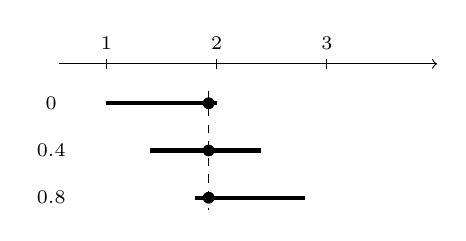
\begin{tikzpicture}[x=1mm,y=1mm,font=\scriptsize]
\draw[->] (14,22) -- (62,22);
\foreach \x/\lab in {20/1,34/2,48/3}
  \draw (\x,21.4) -- (\x,22.6) node[above=0pt]{\lab};
\node[] at (13,17) {$0$};
\draw[line width=1.5pt] (20,17) -- (34,17);
\myvdots{13}{14.7}{0.7}{0.1}
\node at (13,11) {$0.4$};
\draw[line width=1.5pt] (25.6,11) -- (39.6,11);
\myvdots{13}{8.7}{0.7}{0.1}
\node at (13,5) {$0.8$};
\draw[line width=1.5pt] (31.2,5) -- (45.2,5);
\myvdots{13}{2.7}{0.7}{0.1}
\draw[dashed] (33,18.5) -- (33,3.5);
\foreach \y in {17,11,5}
  \fill (33,\y) circle (0.75);
\end{tikzpicture}
\caption{$\kI=[1,2]$}\label{fig:non_punctual}
\end{subfigure}
\hfill
\begin{subfigure}[t]{0.47\textwidth}
\centering
\begin{tikzpicture}[x=1mm,y=1mm,font=\scriptsize]
\draw[->] (14,22) -- (62,22);
\foreach \x/\lab in {20/1,34/2,48/3}
  \draw (\x,21.4) -- (\x,22.6) node[above=0pt]{\lab};
\node at (13,17) {$0$};
\fill (20,17) circle (0.75);
\myvdots{13}{14.7}{0.7}{0.1}
\node at (13,11) {$0.4$};
\fill (25.6,11) circle (0.75);
\myvdots{13}{8.7}{0.7}{0.1}
\node at (13,5) {$0.8$};
\fill (31.2,5) circle (0.75);
\myvdots{13}{2.7}{0.7}{0.1}
\end{tikzpicture}
\caption{$\kI=[1,1]$}\label{fig:punctual}
\end{subfigure}
\caption{Onsets of a persistent demand and their windows.}
\label{fig:punctual_vs_nonpunctual}
\end{figure}

The procedure is sound and terminating for all of TCTL. Completeness is confined to the non-punctual
case, and rests on the single formula-clock: a persistent context re-demands $\mu$ at a continuum of
onsets, and one $x_\mu$ serves them all only because their windows overlap. For $\kI=[a,b]$ with
$a<b$, nearby onsets share a common time (Fig.~\ref{fig:non_punctual}), so the pending obligations
collapse to a single earliest deadline, which is what $x_\mu$ records. For $\kI=[a,a]$
(Fig.~\ref{fig:punctual}) the windows are pairwise disjoint singletons, no witness serves two onsets,
and the obligations a model carries at a given moment depend on the exact offsets of every onset still
pending. Such a model projects onto no finite set of nodes and the repeating segment of
Theorem~\ref{thm:completeness} need not exist: on punctual intervals the procedure still runs and
terminates, but may fail to find a successful marking for a satisfiable formula.

In practice the full generality of TCTL is rarely needed. The common use is properties of temporal
nesting depth at most one --- state reachability, safety and inevitability --- as supported by tools
such as \textsc{Uppaal}~\cite{BehrmannLarsenYi2004Uppaal} and \textsc{Romeo}~\cite{lime-TACAS-09}, the
one exception being the leads-to query. There the continuum of onsets never arises: a modality whose
argument is propositional is demanded once, where \ruleref{Cov} fires, and never re-imposed inside
another pursuit.

\begin{corollary}\label{cor:depthone}
The tableau procedure is sound and complete for TCTL of temporal nesting depth at most one.
\end{corollary}
\begin{proof}
Soundness follows from Theorem~\ref{thm:soundness}. The completeness argument is unchanged up to the
projection step. Fresh onsets arise only when a modality is demanded inside another's pursuit, which
at depth one cannot happen, every argument being propositional. The obligations live at a node are
then exactly the pursuits it carries, all recorded in $\Gamma$, $\Ctx$ and $\Deadline$ with their elapsed time
in $Z$, so a repeat $N_i\equiv N_j$ agrees on the full obligation state and the projection goes
through for every $\kI$.
\end{proof}

\noindent
Leads-to queries, written $\mathrm{AG}(p\rightarrow\mathrm{AF}_\kI q)$, have depth two and fall
outside the corollary, the outer modality re-demanding the inner one at a continuum of onsets. They
remain covered by Theorem~\ref{thm:completeness} whenever $\kI$ is non-punctual.
